\documentclass{ltjsarticle}

\usepackage{amsmath}

\usepackage{tikz}
\usetikzlibrary{calc}
\usetikzlibrary {decorations.pathmorphing,decorations.pathreplacing,decorations.shapes}

 \pagestyle{empty}

\begin{document}

\Huge

\LaTeX でラムダ式を記述するときには空白を調整したほうがよい

調整しない場合以下のようになる\\
\begin{minipage}[t]{0.5\textwidth}
$ \lambda x:T.e $
\end{minipage}
\begin{minipage}[t]{0.5\textwidth}
\verb|\lambda x:T.e|
\end{minipage}

\vspace{5mm}

これは
$
  \begin{tikzpicture}[remember picture,inner sep=0pt] \node (lambda1) {$\lambda$}; \end{tikzpicture}
  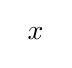
\begin{tikzpicture}[remember picture,inner sep=0pt] \node (x1) {$x$}; \end{tikzpicture}
  \mathrel{\begin{tikzpicture}[remember picture,inner sep=0pt] \node (colon1) {$:$}; \end{tikzpicture}}
  
\begin{tikzpicture}[remember picture,inner sep=0pt] \node (T1) {$T$}; \end{tikzpicture}
  \begin{tikzpicture}[remember picture,inner sep=0pt] \node (dot1) {$.$}; \end{tikzpicture}
  \begin{tikzpicture}[remember picture,inner sep=0pt] \node (e1) {$e$}; \end{tikzpicture}
$
というまとまりにみえてしまう

\begin{tikzpicture}[remember picture,overlay]
  \coordinate (lNW11) at ([yshift=1mm]lambda1.north west);
  \coordinate (lNW12) at ([yshift=3mm]lambda1.north west);
  \draw[decorate,decoration=brace] (lNW11) -- (lNW11 -| x1.east);
  \draw[decorate,decoration=brace] (lNW11 -| T1.west) -- (lNW11 -| e1.east);
  \draw[decorate,decoration=brace] (lNW12) -- (lNW12 -| e1.east);
\end{tikzpicture}


論理的には
$
  \begin{tikzpicture}[remember picture,inner sep=0pt] \node (lambda2) {$\lambda$}; \end{tikzpicture}
  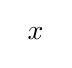
\begin{tikzpicture}[remember picture,inner sep=0pt] \node (x2) {$x$}; \end{tikzpicture}
  \mathrel{\begin{tikzpicture}[remember picture,inner sep=0pt] \node (colon2) {$:$}; \end{tikzpicture}}
  
\begin{tikzpicture}[remember picture,inner sep=0pt] \node (T2) {$T$}; \end{tikzpicture}
  \begin{tikzpicture}[remember picture,inner sep=0pt] \node (dot2) {$.$}; \end{tikzpicture}
  \begin{tikzpicture}[remember picture,inner sep=0pt] \node (e2) {$e$}; \end{tikzpicture}
$
という構造である \\
($T$ 型の引数 $x$ を受け取って $e$ を返す関数、という意味なので、$x$ と $T$ の関係は $T$ と $e$ の関係よりも近い)

\begin{tikzpicture}[remember picture,overlay]
  \coordinate (lNW21) at ([yshift=1mm]lambda2.north west);
  \coordinate (lNW22) at ([yshift=3mm]lambda2.north west);
  \draw[decorate,decoration=brace] (lNW21 -| x2.west) -- (lNW21 -| T2.east);
  \draw[decorate,decoration=brace] (lNW22) -- (lNW22 -| e2.east);
\end{tikzpicture}

\TeX がこのように空白を入れるのは、$:$ が関係演算子であり、
関係演算子の左右には大きめの空白 (thick space) を入れる
という規則になっているためである \\
(詳しい規則は \TeX{}book に載っている)

\newpage

調整しない場合\\
\begin{minipage}[t]{0.2\textwidth}
$ \lambda x:T.e $
\end{minipage}
\begin{minipage}[t]{0.79\textwidth}
\verb|\lambda x:T.e|
\end{minipage}\\

$:$ を関係演算子でなく、普通の文字扱いにすると空白がなくなる\\
\begin{minipage}[t]{0.2\textwidth}
$ \lambda x\mathord{:}T.e $
\end{minipage}
\begin{minipage}[t]{0.8\textwidth}
\verb|\lambda x\mathord{:}T.e|
\end{minipage}\\

\verb|\mathord| を使わずに、ブレースで括るだけでも同じ効果がある\\
\begin{minipage}[t]{0.2\textwidth}
$ \lambda x{:}T.e $
\end{minipage}
\begin{minipage}[t]{0.8\textwidth}
\verb|\lambda x{:}T.e|
\end{minipage}\\

$x$ と $T$ よりも $T$ と $e$ の関係のほうが離れているので、
$e$ の直前に小さな空白 (thin space) を入れることも考えられる \\
これは $.$ を関係演算子でなく、punct にすることで可能 \\
\begin{minipage}[t]{0.2\textwidth}
$ \lambda x{:}T\mathpunct{.}e $
\end{minipage}
\begin{minipage}[t]{0.8\textwidth}
\verb|\lambda x{:}T\mathpunct{.}e|
\end{minipage}\\
(もちろん、\verb|\,| を使う手もある)

\newpage

各文字の種類を調べるには \verb|\showlists| が使える

\Large

\begin{minipage}[t]{0.5\textwidth}
\begin{verbatim}
\documentclass{article}
\tracingonline1
\showboxdepth10000
\showboxbreadth10000
\begin{document}
$ \lambda x:T.e \showlists $
\end{document}
\end{verbatim}
\end{minipage}
\begin{minipage}[t]{0.4\textwidth}
\begin{verbatim}
% latex t.tex
...
### math mode entered at line 6
\mathord
.\fam1 ^^U
\mathord
.\fam1 x
\mathrel
.\fam0 :
\mathord
.\fam1 T
\mathord
.\fam1 :
\mathord
.\fam1 e
...
\end{verbatim}
\end{minipage}

\Huge

(もっとわかりやすいやり方は欲しい)


\end{document}
